% Options for packages loaded elsewhere
% Options for packages loaded elsewhere
\PassOptionsToPackage{unicode}{hyperref}
\PassOptionsToPackage{hyphens}{url}
\PassOptionsToPackage{dvipsnames,svgnames,x11names}{xcolor}
%
\documentclass[
]{article}
\usepackage{xcolor}
\usepackage[left=1in,right=1in,top=1in,bottom=1in]{geometry}
\usepackage{amsmath,amssymb}
\setcounter{secnumdepth}{-\maxdimen} % remove section numbering
\usepackage{iftex}
\ifPDFTeX
  \usepackage[T1]{fontenc}
  \usepackage[utf8]{inputenc}
  \usepackage{textcomp} % provide euro and other symbols
\else % if luatex or xetex
  \usepackage{unicode-math} % this also loads fontspec
  \defaultfontfeatures{Scale=MatchLowercase}
  \defaultfontfeatures[\rmfamily]{Ligatures=TeX,Scale=1}
\fi
\usepackage{lmodern}
\ifPDFTeX\else
  % xetex/luatex font selection
  \setmainfont[]{Latin Modern Roman}
\fi
% Use upquote if available, for straight quotes in verbatim environments
\IfFileExists{upquote.sty}{\usepackage{upquote}}{}
\IfFileExists{microtype.sty}{% use microtype if available
  \usepackage[]{microtype}
  \UseMicrotypeSet[protrusion]{basicmath} % disable protrusion for tt fonts
}{}
\makeatletter
\@ifundefined{KOMAClassName}{% if non-KOMA class
  \IfFileExists{parskip.sty}{%
    \usepackage{parskip}
  }{% else
    \setlength{\parindent}{0pt}
    \setlength{\parskip}{6pt plus 2pt minus 1pt}}
}{% if KOMA class
  \KOMAoptions{parskip=half}}
\makeatother
% Make \paragraph and \subparagraph free-standing
\makeatletter
\ifx\paragraph\undefined\else
  \let\oldparagraph\paragraph
  \renewcommand{\paragraph}{
    \@ifstar
      \xxxParagraphStar
      \xxxParagraphNoStar
  }
  \newcommand{\xxxParagraphStar}[1]{\oldparagraph*{#1}\mbox{}}
  \newcommand{\xxxParagraphNoStar}[1]{\oldparagraph{#1}\mbox{}}
\fi
\ifx\subparagraph\undefined\else
  \let\oldsubparagraph\subparagraph
  \renewcommand{\subparagraph}{
    \@ifstar
      \xxxSubParagraphStar
      \xxxSubParagraphNoStar
  }
  \newcommand{\xxxSubParagraphStar}[1]{\oldsubparagraph*{#1}\mbox{}}
  \newcommand{\xxxSubParagraphNoStar}[1]{\oldsubparagraph{#1}\mbox{}}
\fi
\makeatother


\usepackage{longtable,booktabs,array}
\newcounter{none} % for unnumbered tables
\usepackage{calc} % for calculating minipage widths
% Correct order of tables after \paragraph or \subparagraph
\usepackage{etoolbox}
\makeatletter
\patchcmd\longtable{\par}{\if@noskipsec\mbox{}\fi\par}{}{}
\makeatother
% Allow footnotes in longtable head/foot
\IfFileExists{footnotehyper.sty}{\usepackage{footnotehyper}}{\usepackage{footnote}}
\makesavenoteenv{longtable}
\usepackage{graphicx}
\makeatletter
\newsavebox\pandoc@box
\newcommand*\pandocbounded[1]{% scales image to fit in text height/width
  \sbox\pandoc@box{#1}%
  \Gscale@div\@tempa{\textheight}{\dimexpr\ht\pandoc@box+\dp\pandoc@box\relax}%
  \Gscale@div\@tempb{\linewidth}{\wd\pandoc@box}%
  \ifdim\@tempb\p@<\@tempa\p@\let\@tempa\@tempb\fi% select the smaller of both
  \ifdim\@tempa\p@<\p@\scalebox{\@tempa}{\usebox\pandoc@box}%
  \else\usebox{\pandoc@box}%
  \fi%
}
% Set default figure placement to htbp
\def\fps@figure{htbp}
\makeatother


% definitions for citeproc citations
\NewDocumentCommand\citeproctext{}{}
\NewDocumentCommand\citeproc{mm}{%
  \begingroup\def\citeproctext{#2}\cite{#1}\endgroup}
\makeatletter
 % allow citations to break across lines
 \let\@cite@ofmt\@firstofone
 % avoid brackets around text for \cite:
 \def\@biblabel#1{}
 \def\@cite#1#2{{#1\if@tempswa , #2\fi}}
\makeatother
\newlength{\cslhangindent}
\setlength{\cslhangindent}{1.5em}
\newlength{\csllabelwidth}
\setlength{\csllabelwidth}{3em}
\newenvironment{CSLReferences}[2] % #1 hanging-indent, #2 entry-spacing
 {\begin{list}{}{%
  \setlength{\itemindent}{0pt}
  \setlength{\leftmargin}{0pt}
  \setlength{\parsep}{0pt}
  % turn on hanging indent if param 1 is 1
  \ifodd #1
   \setlength{\leftmargin}{\cslhangindent}
   \setlength{\itemindent}{-1\cslhangindent}
  \fi
  % set entry spacing
  \setlength{\itemsep}{#2\baselineskip}}}
 {\end{list}}
\usepackage{calc}
\newcommand{\CSLBlock}[1]{\hfill\break\parbox[t]{\linewidth}{\strut\ignorespaces#1\strut}}
\newcommand{\CSLLeftMargin}[1]{\parbox[t]{\csllabelwidth}{\strut#1\strut}}
\newcommand{\CSLRightInline}[1]{\parbox[t]{\linewidth - \csllabelwidth}{\strut#1\strut}}
\newcommand{\CSLIndent}[1]{\hspace{\cslhangindent}#1}



\setlength{\emergencystretch}{3em} % prevent overfull lines

\providecommand{\tightlist}{%
  \setlength{\itemsep}{0pt}\setlength{\parskip}{0pt}}



 


\usepackage{booktabs}
\usepackage{longtable}
\usepackage{array}
\usepackage{multirow}
\usepackage{wrapfig}
\usepackage{float}
\usepackage{colortbl}
\usepackage{pdflscape}
\usepackage{tabu}
\usepackage{threeparttable}
\usepackage{threeparttablex}
\usepackage[normalem]{ulem}
\usepackage{makecell}
\usepackage{xcolor}
\usepackage[font=footnotesize]{caption}
\usepackage[noblocks]{authblk}
\renewcommand*{\Authsep}{, }
\renewcommand*{\Authand}{, }
\renewcommand*{\Authands}{, }
\renewcommand\Affilfont{\small}
\renewcommand{\thefootnote}{\alph{footnote}}
\usepackage{etoolbox}
\AtEndEnvironment{abstract}{\noindent\textbf{Keywords:} \KeywordList \par}
\makeatletter
\@ifpackageloaded{caption}{}{\usepackage{caption}}
\AtBeginDocument{%
\ifdefined\contentsname
  \renewcommand*\contentsname{Table of contents}
\else
  \newcommand\contentsname{Table of contents}
\fi
\ifdefined\listfigurename
  \renewcommand*\listfigurename{List of Figures}
\else
  \newcommand\listfigurename{List of Figures}
\fi
\ifdefined\listtablename
  \renewcommand*\listtablename{List of Tables}
\else
  \newcommand\listtablename{List of Tables}
\fi
\ifdefined\figurename
  \renewcommand*\figurename{Figure}
\else
  \newcommand\figurename{Figure}
\fi
\ifdefined\tablename
  \renewcommand*\tablename{Table}
\else
  \newcommand\tablename{Table}
\fi
}
\@ifpackageloaded{float}{}{\usepackage{float}}
\floatstyle{ruled}
\@ifundefined{c@chapter}{\newfloat{codelisting}{h}{lop}}{\newfloat{codelisting}{h}{lop}[chapter]}
\floatname{codelisting}{Listing}
\newcommand*\listoflistings{\listof{codelisting}{List of Listings}}
\makeatother
\makeatletter
\usepackage{pdflscape}
\makeatother
\makeatletter
\makeatother
\makeatletter
\@ifpackageloaded{caption}{}{\usepackage{caption}}
\@ifpackageloaded{subcaption}{}{\usepackage{subcaption}}
\makeatother
\usepackage{bookmark}
\IfFileExists{xurl.sty}{\usepackage{xurl}}{} % add URL line breaks if available
\urlstyle{same}
\hypersetup{
  pdftitle={Names of resistance exercises: text analysis of survey responses},
  pdfauthor={James L. Nuzzo; James Steele},
  pdfkeywords={language, linguistics, nomenclature, resistance
exercise, strength training, taxonomy, terminology},
  colorlinks=true,
  linkcolor={blue},
  filecolor={Maroon},
  citecolor={Blue},
  urlcolor={Blue},
  pdfcreator={LaTeX via pandoc}}


\title{Names of resistance exercises: text analysis of survey
responses\thanks{Preprint, please cite as: Nuzzo, J.L., and Steele, J.
(2026). Names of resistance exercises: text analysis of survey
responses. sportrxiv DOI: \url{https://doi.org/10.51224/SportRxiv.872}.
Addresses for correspondence: jameslnuzzo@gmail.com;
james@steele-research.com}}


\author[1]{James L. Nuzzo}
\author[2,3,4]{James Steele}

\affil[1]{The Nuzzo Letter, West Leederville, Western Australia,
Australia}
\affil[2]{Steele Research Limited, Eastleigh, Hampshire, UK}
\affil[3]{MacroFactor, Stronger by Science Technologies LLC, Raleigh,
North Carolina, USA}
\affil[4]{School of Health and Biomedical Sciences, Royal Melbourne
Institute of Technology, Melbourne, VIC, Australia}

% Store the keywords (expanded by Pandoc here)
\def\KeywordList{language, linguistics, nomenclature, resistance
exercise, strength training, taxonomy, terminology}

\date{May 15, 2026}
\begin{document}
\maketitle
\begin{abstract}
Names of resistance exercises play an important role in education and
promoting exercise participation. Yet, previous research has documented
that exercises are named inconsistently among exercise professionals and
within exercise textbooks and journal articles. Greater standardization
or the development of a taxonomy may therefore be warranted, but
large-scale data on naming practices are limited. This study examined
how resistance exercises are named in a large sample. A total of 1,849
individuals completed an online survey; analyses were restricted to
1,425 respondents who passed attention checks and reported English as
their primary exercise-related language. Participants were predominantly
male (76\%), highly educated (82\% held a Bachelor's degree or higher;
42\% in exercise-related fields), and experienced in resistance training
(median 10 years {[}IQR: 5--15{]}). Nearly half of respondents held
relevant certifications (46\%) or had worked in resistance training
instruction (49\%). Respondents viewed images of exercises performed
with free weights, traditional machines, and a connected adaptive
resistance machine. Respondents indicated whether they recognised the
exercise in each image and what they call the exercise. Text analyses
examined word frequencies, term-frequency--inverse exercise frequency
(tf-ief), and common bigrams. Most exercises were widely recognised
(\textgreater90\% of respondents), except those using connected adaptive
machines (62.3--67.3\% of respondents). Recognition influenced naming
patterns: respondents who recognised exercises used more consistent,
commonly shared terminology, whereas respondents who did not recognise
exercises used more idiosyncratic naming. Equipment-related terms were
consistently important, but other naming components (e.g., body
position, body part, movement direction, unilateral/bilateral execution)
varied substantially in importance. Bigrams showed that recognised
exercises were typically labelled using ``textbook'' word pairings,
while unrecognised exercises produced more variable combinations.
Participants generally agreed that exercise names are important (74\%),
inconsistently used (63\%), and influence learning (69\%). Many
respondents reported using multiple names for the same exercise (73\%),
and most respondents supported standardization of exercise names (69\%).
Overall, the findings suggest that exercise naming follows broad
linguistic principles (e.g., Zipf's law) but also highlight elements of
a shared ``folk taxonomy''. Despite this, there was substantial
inconsistency in resistance exercise naming practices. However, whilst
such a folk taxonomy might enable clear communication within public and
applied settings, the development of standardized terminology or a
formal scientific taxonomy might ensure that cross-communication and
understanding across domains is more easily achieved. Alternatively, a
hierarchical taxonomy and system of translation across synonyms in use
already may be a valuable pursuit.
\end{abstract}


\section{Introduction}\label{introduction}

Movement patterns performed in resistance exercise programs are given
names to facilitate communication and understanding of resistance
exercise in both applied and scientific settings. Ideally, each
resistance exercise would have a unique name, and this name would
distinguish it from all other exercises, leading to a clear, cohesive,
accurate, and consistent taxonomy of exercise names; or at the very
least there would be shared understanding if synonyms are used as
lexical labels.

Limited descriptive research on use of exercise names exists (Jackson et
al., 2013; Nuzzo, 2017, 2021). Of existing studies, all have documented
that resistance exercises are named inconsistently in a range of
settings and populations suggesting a lack of a shared taxonomy (Jackson
et al., 2013; Nuzzo, 2017, 2021). Jackson et al. (2013) found that
exercises are named inconsistently within and between individuals
employed in various exercise-related professions (e.g., personal
trainers, strength and conditioning coaches, athletic trainers, exercise
academics). In previous work, the lead author (Nuzzo, 2017, 2021) found
that resistance exercises are named inconsistently in textbooks and
research articles. Additionally, the author revealed that exercise names
consist of various types of words (e.g., action words, action direction
words, body part words, body position words, equipment words, equipment
position words) and that the way that these words are organized in
exercise names (i.e., naming patterns) is inconsistent (Nuzzo, 2017).

An inconsistent exercise nomenclature is problematic because of its
potential to lead to diminished communication efficiency and efficacy.
For example, the phrases ``heel raise'' and ``calf raise'' are used to
refer to the same exercise, as are the phrases ``arm curl'' and ``biceps
curl'' (Nuzzo, 2021); yet, this confusion seems unnecessary and
resolvable (see Jackson et al. (2013), Nuzzo (2017), and Nuzzo (2021),
for more examples). Consequently, some researchers have made normative
claims that exercise names should be standardized (Jackson et al., 2013;
Nuzzo, 2017, 2021; Nuzzo \& Nosaka, 2023). A standardized system of
exercise names would perhaps not be too dissimilar to taxonomic and
nomenclature systems that have been developed in other fields of biology
(Winston, 2018). However, even in other fields there are often both folk
and scientific taxonomies in use concomitantly by different groups i.e.,
lay people, applied practitioners, and scientists (Berlin, 1972; Berlin
et al., 1973; Brown et al., 1976). Whilst within groups a shared
taxonomy that differs from other groups may still enable clear
communication to take place, for an applied scientific field such as
exercise science, where there is often cross-communication between both
groups, inconsistency has the potential to hamper communication and
shared understanding.

A move toward standardization will present challenges, particularly
given the present degree of inconsistency shown in descriptive research
(Jackson et al., 2013; Nuzzo, 2017, 2021). For example, there are
various types of words that make up exercise names (Jackson et al.,
2013; Nuzzo, 2017, 2021; Nuzzo \& Nosaka, 2023), and no consensus has
been reached regarding what exercise naming pattern, if any, should be
adopted, and what rules should be followed in naming exercises (Jackson
et al., 2013; Nuzzo, 2017). Further, the extent to which scientists
should adopt their own scientific taxonomy vs adopting any emergent folk
taxonomy in use by the public and/or practitioners as a result of
typical principles of natural language use (e.g., Zipf's law) is unclear
in terms of how easily either would facilitate communication. Given the
large scope of the problem, there is still a relative lack of data.
Previous studies have been limited to a relatively small number of
exercises, a small number of survey responders, and a narrowed focus of
content, such as only examining naming by practitioners and in student
textbooks or research articles (Jackson et al., 2013; Nuzzo, 2017,
2021).

To the extent that standardization of exercise names might be possible,
an informative next step would be to understand how a large sample of
individuals name various exercises. Therefore, the purpose of the
current study was to explore how exercises are named in a large sample,
including individuals who are employed in the fitness industry and
individuals who are employed outside the fitness industry. Specifically,
our aims were to (a) determine how recognisable specific resistance
exercises are to people, (b) identify the types of words used to name
those exercises, and (c) identify exercise naming patterns.

\section{Methods}\label{methods}

\subsection{Sample and recruitment}\label{sample-and-recruitment}

Multiple strategies were used to recruit survey respondents. First, in
October of 2021, an advertisement to the survey was included in a
newsletter sent out by a fitness equipment company (Vitruvian, West
Perth, Australia) to their email list\footnote{At the time JN was
  employed by Vitruvian, hence having access to enable survey
  distribution via their email list.}. This advertisement resulted in 40
respondents. Second, in October of 2021, an advertisement to the survey
was included in the National Strength and Conditioning Association's
(NSCA) certification newsletter (approximately 50,000 subscribers). This
advertisement resulted in 239 respondents. Third, in November of 2021,
an advertisement to the survey was posted on social media, primarily on
Twitter and Instagram. This advertisement resulted in 1,570 respondents.

\subsection{Survey}\label{survey}

A survey was developed and hosted online (Qualtrics XM, Qualtrics
International Inc., Provo, Utah, United States) (Supplementary File 1).
The online survey consisted of an initial cover letter which described
the survey's aims and procedures. The survey was approved by the Human
Research Ethics Committee at Edith Cowan University (2021-02687-NUZZO).
To proceed with the survey, respondents were required to check an item
indicating that they consent to participate and are 18 years of age or
older. If individuals consented to participate in the survey, they
proceeded to questions about sex, age, country of residence, primary
language spoken, highest level of education completed, occupation type,
and resistance exercise experience. Participants then completed
questions about exercise names. Participants were shown two or more
photographs of a given exercise and asked, \emph{``Do you recognise this
exercise?''} Irrespective of whether participants answered ``yes'' or
``no'' to this question, they then proceeded to a question that asked
them to name the exercise: \emph{``What do you personally call this
exercise? If you are unsure or do not recognise the exercise, what is
your best guess as to what this exercise is called? Type your answer in
the space below.''} Participants were asked to answer these questions
for 25 different exercises, 21 of which were acquired from the National
Strength and Conditioning Associations Essentials of Strength Training
and Conditioning 4th edition textbook (National Strength and
Conditioning Association (NSCA), 2016). The other four photographs were
acquired from the exercise database for the Vitruvian (a connected
adaptive resistance exercise machine; see Nuzzo et al. (2023)). The
stock photos of each exercise were used with permission\footnote{Unfortunately
  we were not afforded permission to reproduce the images outside of the
  survey and so cannot include them for reference here. Readers will
  need to view them in the original source material i.e., National
  Strength and Conditioning Associations Essentials of Strength Training
  and Conditioning 4th edition textbook (National Strength and
  Conditioning Association (NSCA), 2016).} and displayed to survey
respondents. A diverse set of exercises, which involved different body
areas, body positions, joint actions, and equipment, were selected.
Finally, using a five-point Likert scale, participants were asked how
strongly they agree with the following statements about exercise names:
\emph{``Exercise names are important''}; \emph{``Exercises are named
inconsistently''}; \emph{``Exercise names impact how information about
exercise is learned''}; \emph{``I sometimes call the same exercise by
different names''}; and \emph{``A system that standardizes exercise
names would be beneficial.''} For all survey questions, participants
were required to provide a response before proceeding to the next
question.

\subsection{Text Analysis}\label{text-analysis}

All code utilised for data preparation and analyses are available in
either the Open Science Framework page for this project
\url{https://osf.io/4uaqr/} or the corresponding GitHub repository
\url{https://github.com/jamessteeleii/exercise_names_survey}. We cite
all software and packages used in the analysis pipeline using the
\texttt{grateful} package ({Rodriguez-Sanchez et al.}, 2023) which can
be seen here: \url{https://osf.io/n6cqt}. The project was not
pre-registered and all analyses are presented as exploratory and
descriptive.

We focused our exploration primarily on word frequency based analyses of
tokens as both single words and as bigrams (i.e., pairs of consecutive
words) where the latter was used to understand how different word
pairings were typically used. Spelling errors were corrected using the
\texttt{hunspell} spell checker library and then manually checked for
any obvious errors which were manually corrected (see
\texttt{convert\_to\_tokens()} and \texttt{convert\_to\_bigrams()}
functions in the \texttt{functions.R} script:
\url{https://osf.io/7nj6d}. Where double barrel terms were used these
were split into unique words, and all pluralized terms were
singularized.

We began by examining the term frequency of words calculated as
\(\frac{n_{word}}{n_{total}}\) and also visualised the linear
relationship of term frequency on the log10 scale conditioned on the
ranking of that term on the log10 scale (i.e., whether the terms in our
corpus of text conform to Zipf's law that the frequency a word appears
is inversely proportional to its rank). Term frequency was examined by
whether or not an exercise was recognised or not, by specific exercises,
and by their combination to identify whether or not there were
idiosyncrasies in word usage conditioned on these variables. For those
who recognised the exercises we also adapted the term frequency-inverse
document frequency (tf-idf) statistic typically used in textual analysis
to understand the importance of a word to a particular document in a
collection (or corpus) of documents, to instead explore the importance
of specific words to particular exercises examined which could instead
be called the term-frequency-inverse exercise frequency (tf-ief)
calculated for each word as:
\(\left(\frac{n_{word}}{n_{total}}\right)\times ln \left(\frac{n_{exercises}}{n_{exercises\ containing\ word}}\right)\).
Higher values of tf-ief identify particular words as being particularly
important for naming a given exercise. In addition to this we also coded
each exercise based on word types including body position, body part,
action performed, the direction of the action performed, equipment used,
and whether the exercise was bilateral or unilaterally performed, and
then calculated similar statistics with exercises grouped by words
within these word type categories. These additional statistics for each
category were calculated similarly as the tf-ief noted above instead
swapping the subscript \(exercises\) for each of the different word type
categories noted. With respect to our textual analyses we finally
examined the frequencies at which different bigrams were used for
specific exercises conditioned on whether participants recognised the
exercises or not and visualised the networks of the top five bigrams
used. Lastly, we visualised the proportions of participants responding
to different categories on the 5-point Likert scale (ranging ``Strongly
disagree'', ``Disagree'', ``Neutral'', ``Agree'', and ``Strongly
agree'') including the total proportions of negative and positive
responses (i.e., those ``Strongly disagree'' and ``Disagree'', or
``Agree'' and ``Strongly agree'' respectively).

\section{Results}\label{results}

From the responses that we obtained we initially filtered out any that
failed the attention check and also any for whom English was not their
primary language for discussing exercise. Thus, our total sample size
for analyses was 1425 across the three distribution methods (NSCA
certification newsletter = 219, social media = 1170, Vitruvian email
list = 36). The demographic characteristics for the full sample can be
seen in Table~\ref{tbl-demographics}.

\begin{longtable}[t]{ll}

\caption{\label{tbl-demographics}Demographic characteristics for full
sample.}

\tabularnewline

\toprule
Characteristic & Summary\\
\midrule
\addlinespace[0.3em]
\multicolumn{2}{l}{Biological sex}\\
\hspace{1em}\hspace{1em}Female & 343 (24\%)\\
\hspace{1em}\hspace{1em}Male & 1,082 (76\%)\\
Age (years) & 31 (26, 40)\\
\addlinespace[0.3em]
\multicolumn{2}{l}{Highest level of education}\\
\hspace{1em}\hspace{1em}Associate degree & 78 (5.5\%)\\
\hspace{1em}\hspace{1em}Bachelor's degree & 557 (39\%)\\
\hspace{1em}\hspace{1em}High school diploma or GED & 163 (11\%)\\
\hspace{1em}\hspace{1em}Master's degree & 404 (28\%)\\
\hspace{1em}\hspace{1em}PhD or other doctoral degree & 207 (15\%)\\
\hspace{1em}\hspace{1em}Some high school & 16 (1.1\%)\\
University-level qualification in a field related to exercise, physical activity, or sport? & 593 (42\%)\\
Typical resistance training frequency (days) & 4.00 (3.00, 5.00)\\
Resistance training experience (years) & 10 (5, 15)\\
Participated in a weightlifting, powerlifting, or strongman competition? & 388 (27\%)\\
Participated in a bodybuilding competition or other physique-based competition? & 74 (5.2\%)\\
Ever employed in a job involving instruction and/or prescription of resistance training & 703 (49\%)\\
Holds a certification/license qualifying instruction and/or prescription of resistance training & 653 (46\%)\\
Instructed and/or prescribed resistance training for athletes & 526 (37\%)\\
Instructed and/or prescribed resistance training for the general population & 773 (54\%)\\
Instructed and/or prescribed resistance training for clinical populations & 290 (20\%)\\
Never instructed and/or prescribed resistance training & 559 (39\%)\\
\addlinespace[0.3em]
\multicolumn{2}{l}{Current or most recent job role}\\
\hspace{1em}\hspace{1em}Athletic trainer & 20 (1.4\%)\\
\hspace{1em}\hspace{1em}Exercise physiologist & 38 (2.7\%)\\
\hspace{1em}\hspace{1em}Other (type job in the space provided) & 765 (54\%)\\
\hspace{1em}\hspace{1em}Personal trainer & 194 (14\%)\\
\hspace{1em}\hspace{1em}Physical education school teacher & 13 (0.9\%)\\
\hspace{1em}\hspace{1em}Physiotherapist / physical therapist & 78 (5.5\%)\\
\hspace{1em}\hspace{1em}Sports coach & 17 (1.2\%)\\
\hspace{1em}\hspace{1em}Sports scientist & 18 (1.3\%)\\
\hspace{1em}\hspace{1em}Strength and conditioning coach & 128 (9.0\%)\\
\hspace{1em}\hspace{1em}University professor or researcher in one of the above areas & 124 (8.7\%)\\
\hspace{1em}\hspace{1em}Weightlifting or powerlifting coach & 30 (2.1\%)\\
\bottomrule
\multicolumn{2}{l}{\rule{0pt}{1em}\textit{Note: }}\\
\multicolumn{2}{l}{\rule{0pt}{1em}Count data presented as n (\%); continous data presented as median (Q1, Q3)}\\

\end{longtable}

The majority of exercises were recognised by over 90\% of respondents
except for the four exercises performed on the connected adaptive
resistance exercise machine (\textasciitilde62\% to 67\%). The
percentage of respondents who did and did not (excluding non-responses)
recognise each exercise is shown in Table~\ref{tbl-recognise}.

\begin{longtable}[t]{lll}

\caption{\label{tbl-recognise}Percentage of respondents who did and did
not recognise each exercise (ordered by percentage recognised).}

\tabularnewline

\toprule
Exercise & Did not recognise & Recognised\\
\midrule
Barbell Biceps Curl & 0.1\% & 99.9\%\\
Flat Barbell Bench Press & 0.1\% & 99.9\%\\
Hip Sled (Machine) & 0.2\% & 99.8\%\\
Leg (Knee) Extension (Machine) & 0.2\% & 99.8\%\\
Lat Pulldown (Machine) & 0.3\% & 99.7\%\\
\addlinespace
Back Squat & 0.4\% & 99.6\%\\
Incline Dumbbell Bench Press & 0.4\% & 99.6\%\\
One-Arm Dumbbell Row & 0.5\% & 99.5\%\\
Seated Barbell Shoulder Press & 0.6\% & 99.4\%\\
Lateral Shoulder Raise & 0.7\% & 99.3\%\\
\addlinespace
Pec Deck (Machine) & 1.1\% & 98.9\%\\
Bent-Over Row & 1.2\% & 98.8\%\\
Flat Dumbbell Fly & 1.2\% & 98.8\%\\
Hammer Curl & 1.4\% & 98.6\%\\
Standing Calf (Heel) Raise (Machine) & 1.6\% & 98.4\%\\
\addlinespace
Shoulder Press (Machine) & 1.7\% & 98.3\%\\
Upright Row & 1.8\% & 98.2\%\\
Vertical Chest Press (Machine) & 1.8\% & 98.2\%\\
Seated Row (Machine) & 2.5\% & 97.5\%\\
Seated Calf (Heel) Raise (Machine) & 5.8\% & 94.2\%\\
\addlinespace
Wrist Curl & 8.1\% & 91.9\%\\
Vitruvian Back Squat With Bar & 32.7\% & 67.3\%\\
Vitruvian Bench Press With Bar & 33.6\% & 66.4\%\\
Vitruvian Bent-Over Row With Bar & 35.4\% & 64.6\%\\
Vitruvian Biceps Curl With Bar & 37.7\% & 62.3\%\\
\bottomrule

\end{longtable}

Exercise recognition impacted term frequency distribution which can be
seen in Figure~\ref{fig-recognise-freq-plot}. The lack of long right
tails suggests there are common words used by those who recognised the
exercises, yet the absence of this for those who did not recognise them
suggests that there are perhaps more idiosyncratic words being used to
name exercises. This pattern appears also across exercises conditioned
on recognition (see \url{https://osf.io/fgyeb}).

\begin{figure}

\centering{

\pandocbounded{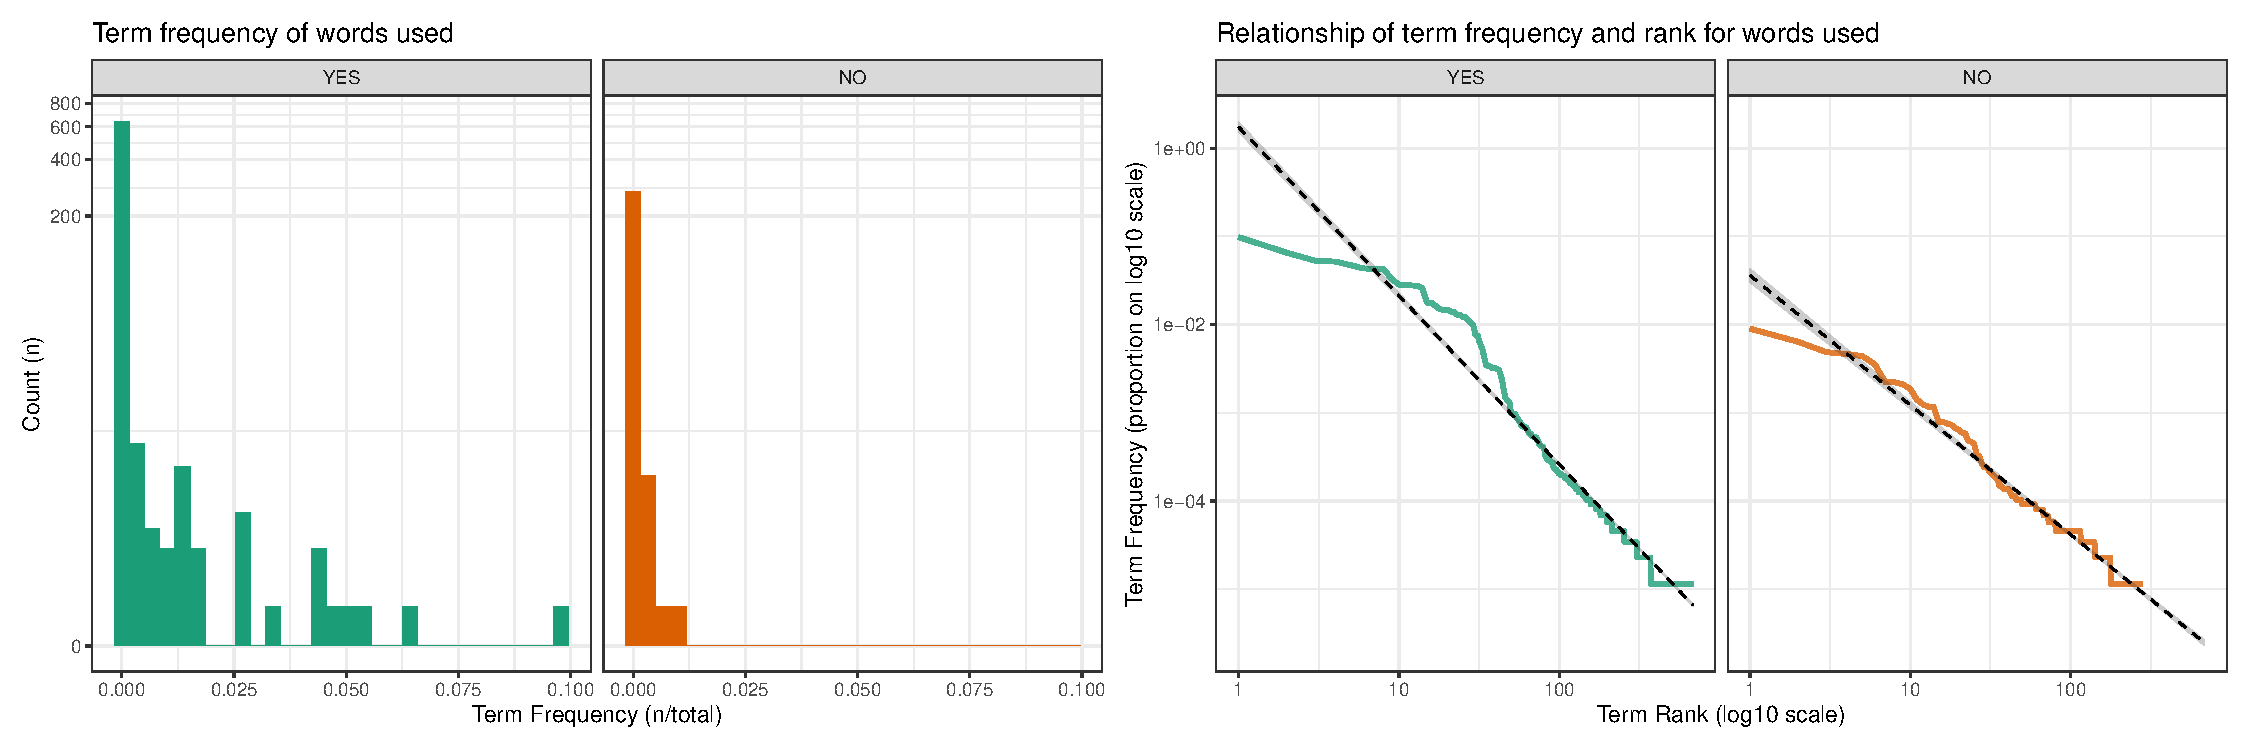
\includegraphics[keepaspectratio]{pre_print_files/figure-pdf/fig-recognise-freq-plot-1.pdf}}

}

\caption{\label{fig-recognise-freq-plot}Term frequencies, and
relationship between term frequency and rank for words used conditioned
on whether an exercise was recognised (``YES'') or not (``NO'').}

\end{figure}%

What specific words were most important for naming particular exercises
can be examined by the tf-ief statistic in Figure~\ref{fig-tf-ief-plot}.
In most cases respondents recognising the exercises used terms that were
indeed used in the ``textbook'' naming conventions for each exercise.
The additional term frequency - inverse word category frequencies can be
seen in the supplementary materials for body position (see
\url{https://osf.io/9n7dm}), body part (see \url{https://osf.io/6d7am}),
action performed (see\url{https://osf.io/23ngw}), the direction of the
action performed (see \url{https://osf.io/9a5wv}), equipment used (see
\url{https://osf.io/c2zpj}), and whether the exercise was bilateral or
unilaterally performed (see \url{https://osf.io/7rmjb}). With the
exception of equipment used, where it was clear that terms accurately
identifying the equipment were most important when naming an exercise
which used that equipment, there was considerable variety in whether
terms relating to the word categories exercises were grouped by were
important when naming them or not.

The pairings of consecutive words used (bigrams) when naming exercises
for those who recognised the exercise can be seen in
Figure~\ref{fig-bigram-recognise-plot}, and for those who did not
recognise the exercise in Figure~\ref{fig-bigram-not-recognise-plot}.
Those who recognised the exercise typically used pairs of words, or
indeed sequences of pairs of words, that reflected the ``textbook''
naming convention for the exercises. However, pairs of words used are
more idiosyncratic for those not recognising the exercise further
supporting the distribution of term frequencies shown above.

\begin{landscape}

\begin{figure}

\centering{

\pandocbounded{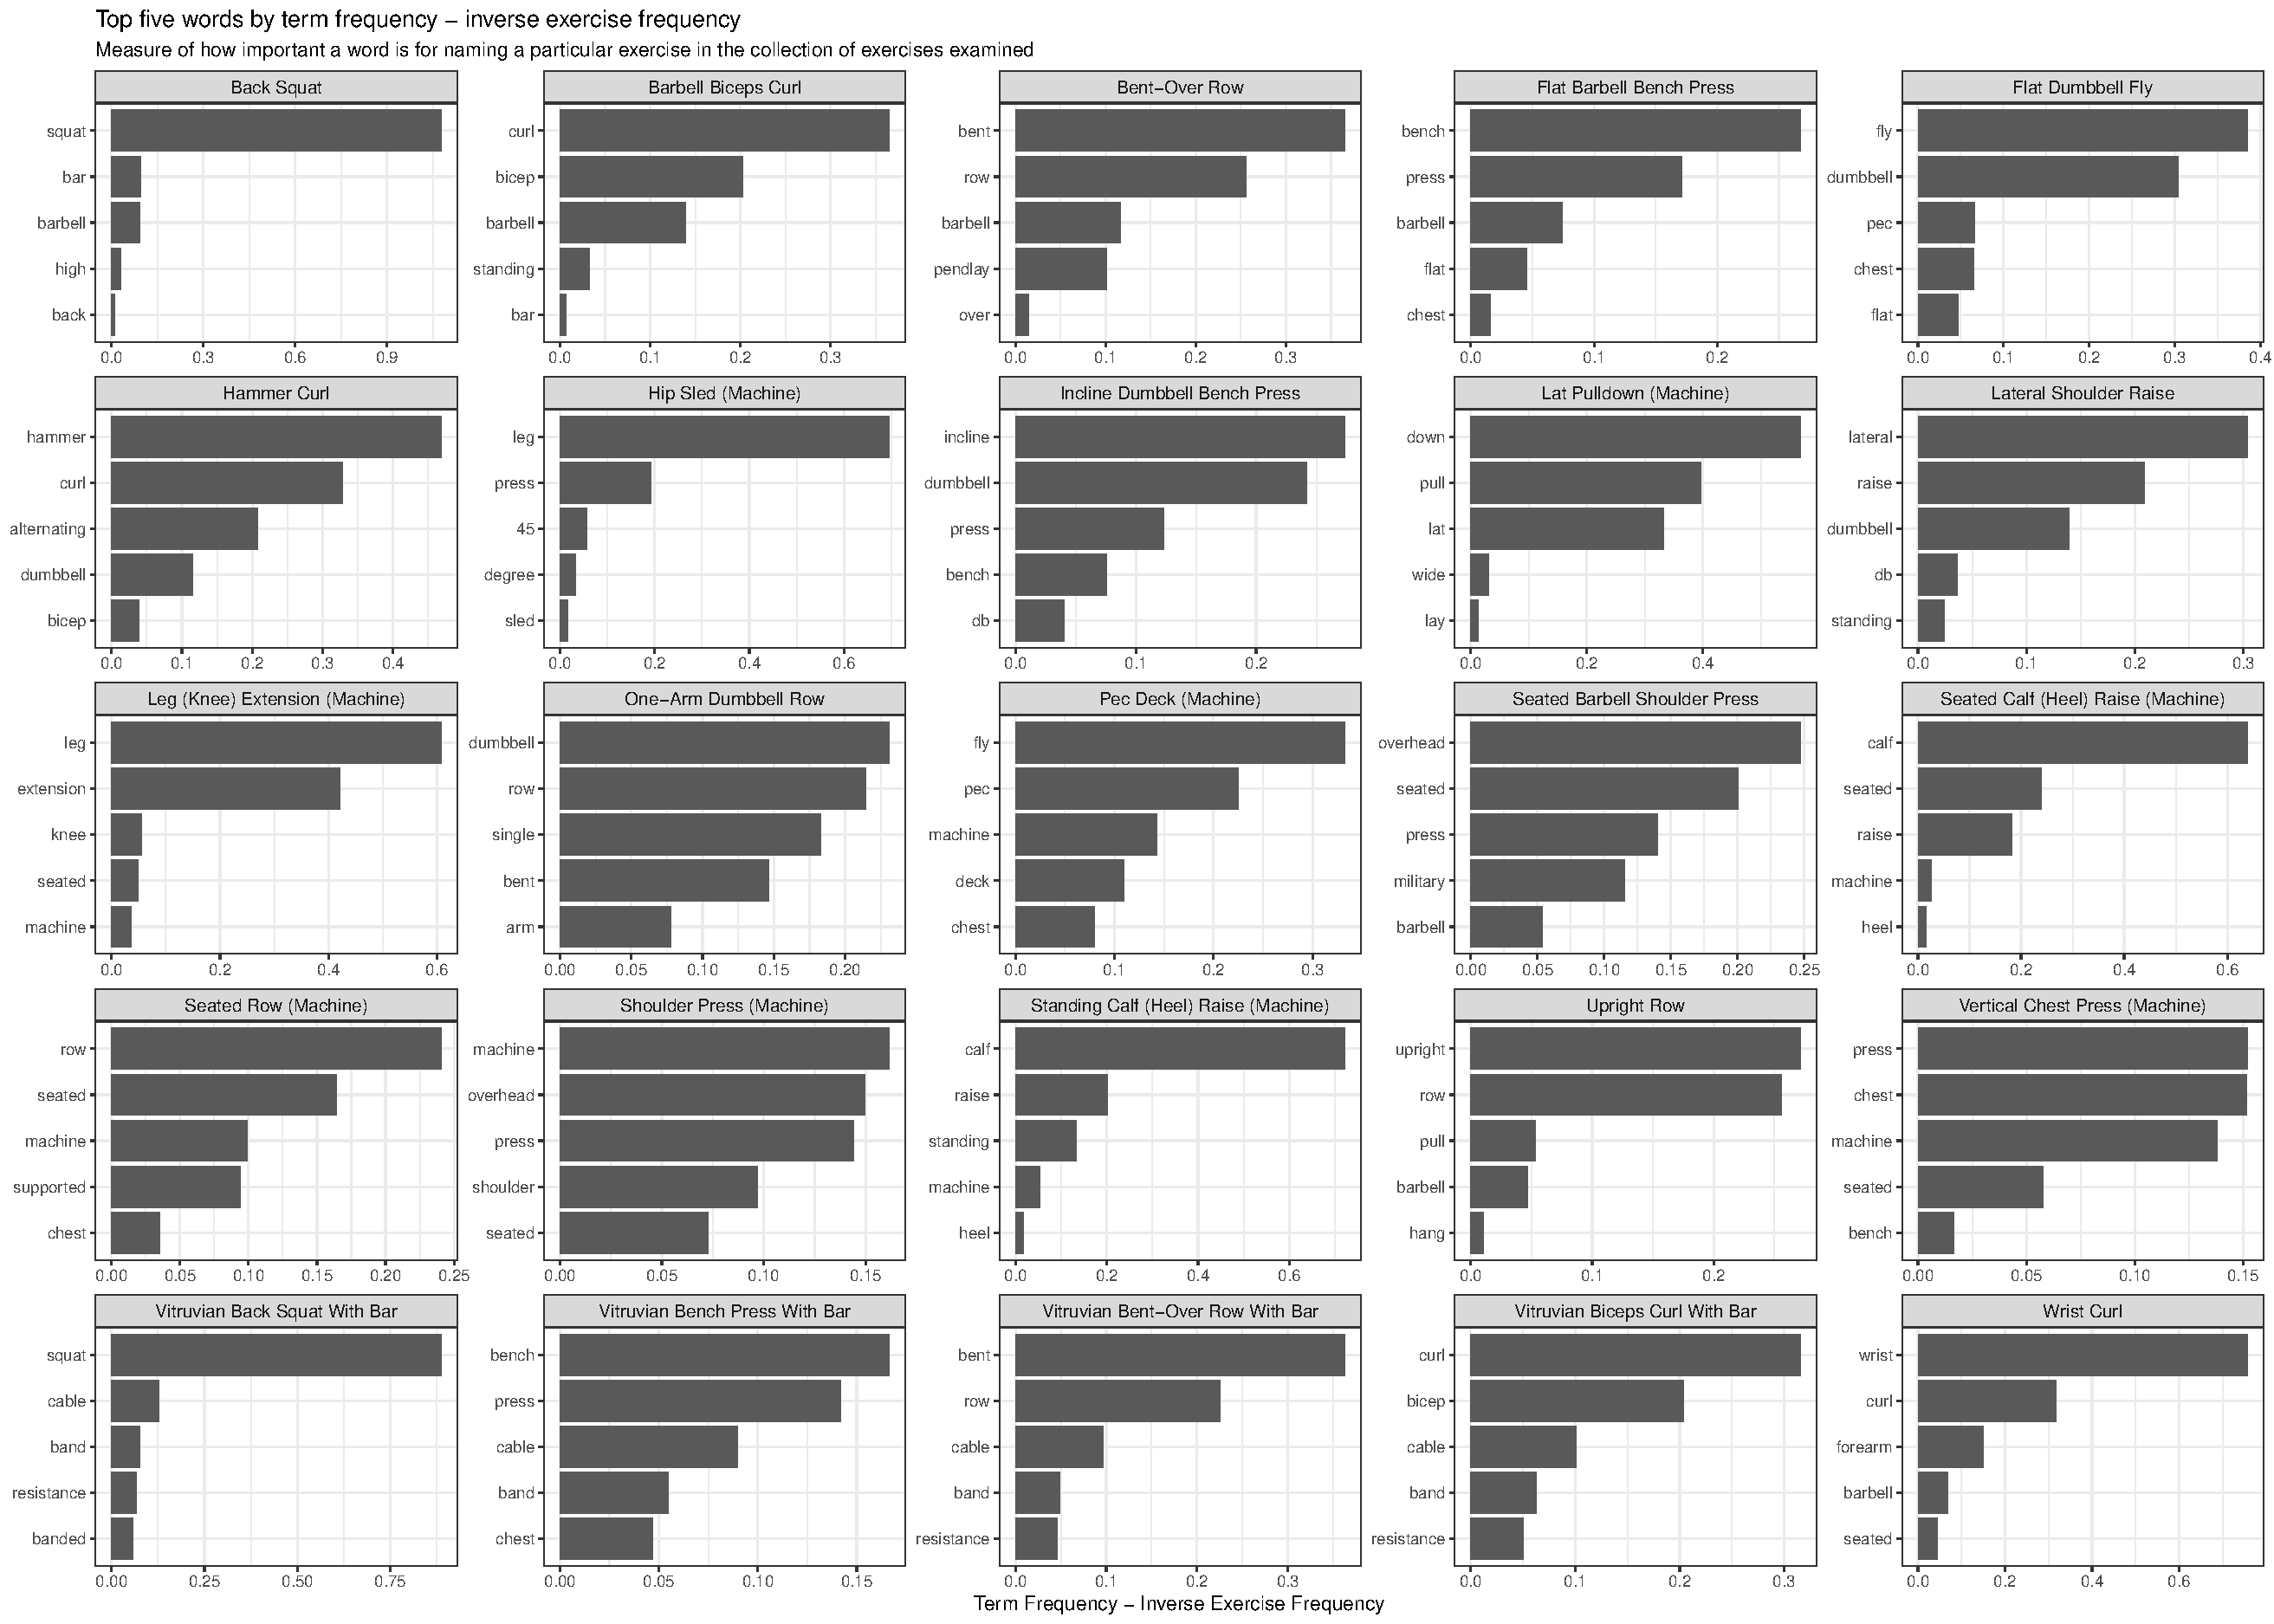
\includegraphics[keepaspectratio]{pre_print_files/figure-pdf/fig-tf-ief-plot-1.pdf}}

}

\caption{\label{fig-tf-ief-plot}Term frequency - inverse exercise
frequency (tf-ief) indicating how imporant specific words are for naming
particular exercises (note, names for exercises on each panel are the
``textbook'' names provided).}

\end{figure}%

\begin{figure}

\centering{

\pandocbounded{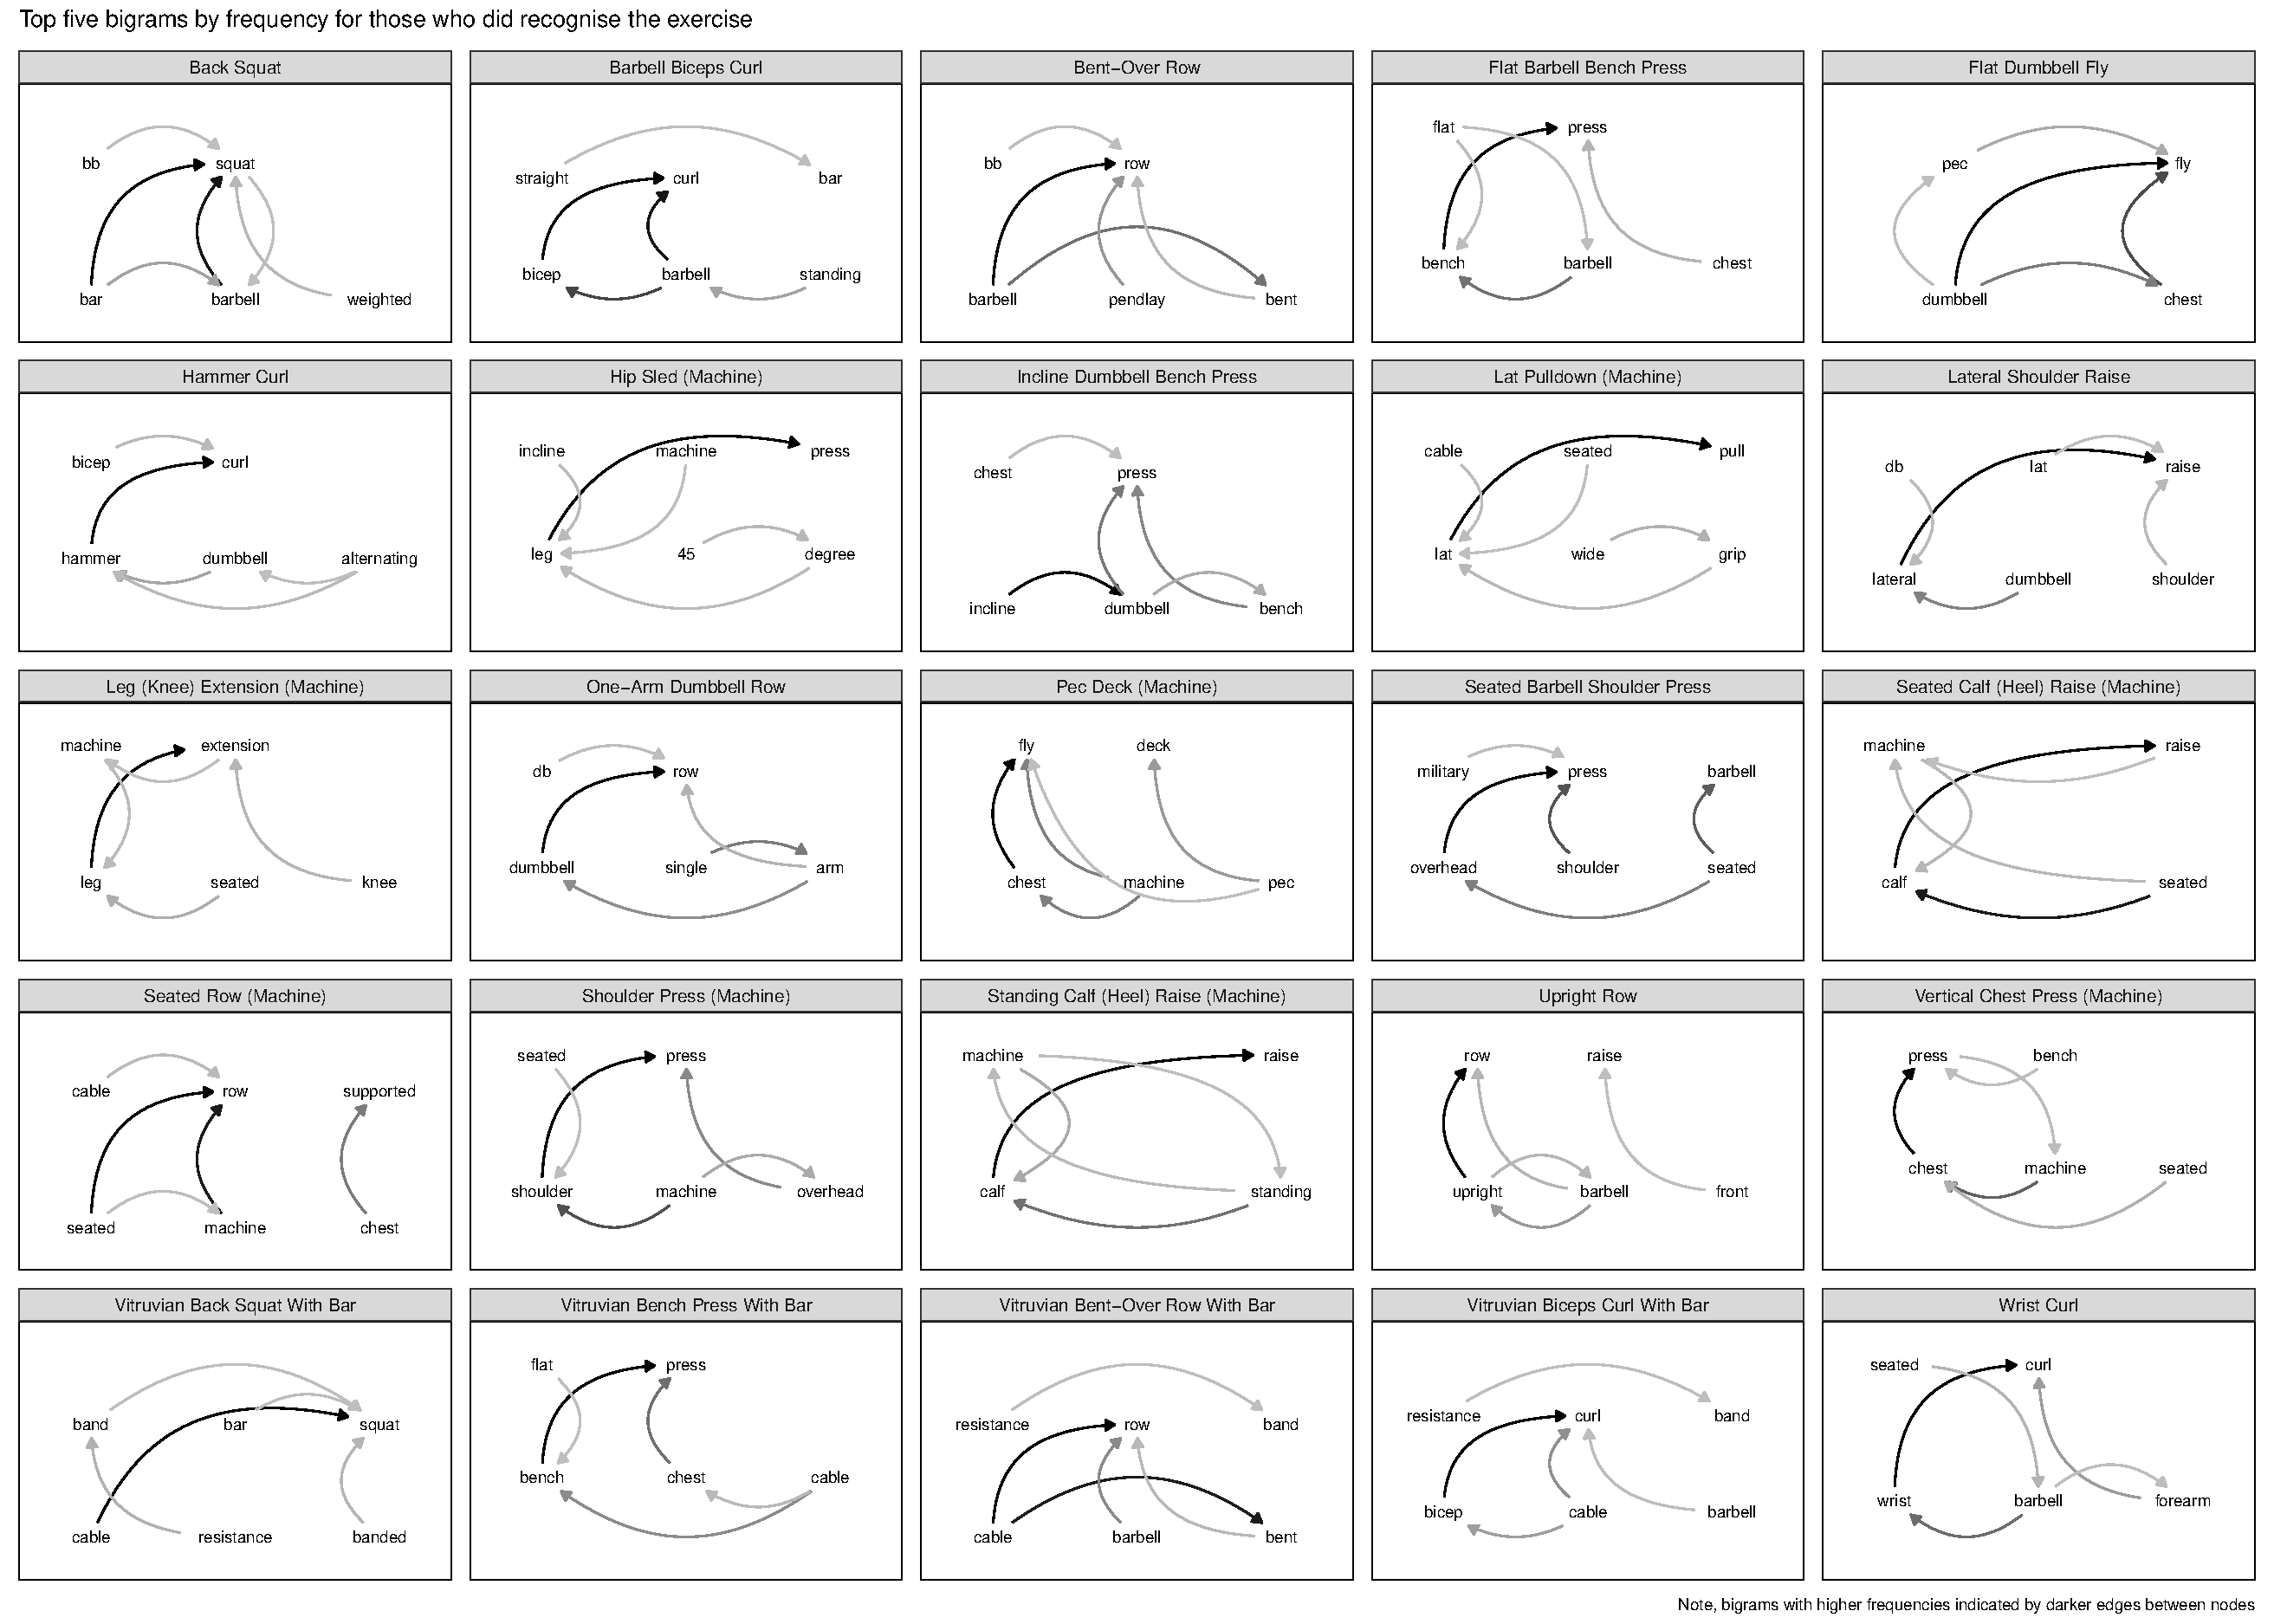
\includegraphics[keepaspectratio]{pre_print_files/figure-pdf/fig-bigram-recognise-plot-1.pdf}}

}

\caption{\label{fig-bigram-recognise-plot}Pairs of consecutive words
(bigrams) used in naming exercises by those who did recognise the
exercise (note, names for exercises on each panel are the ``textbook''
names provided).}

\end{figure}%

\begin{figure}

\centering{

\pandocbounded{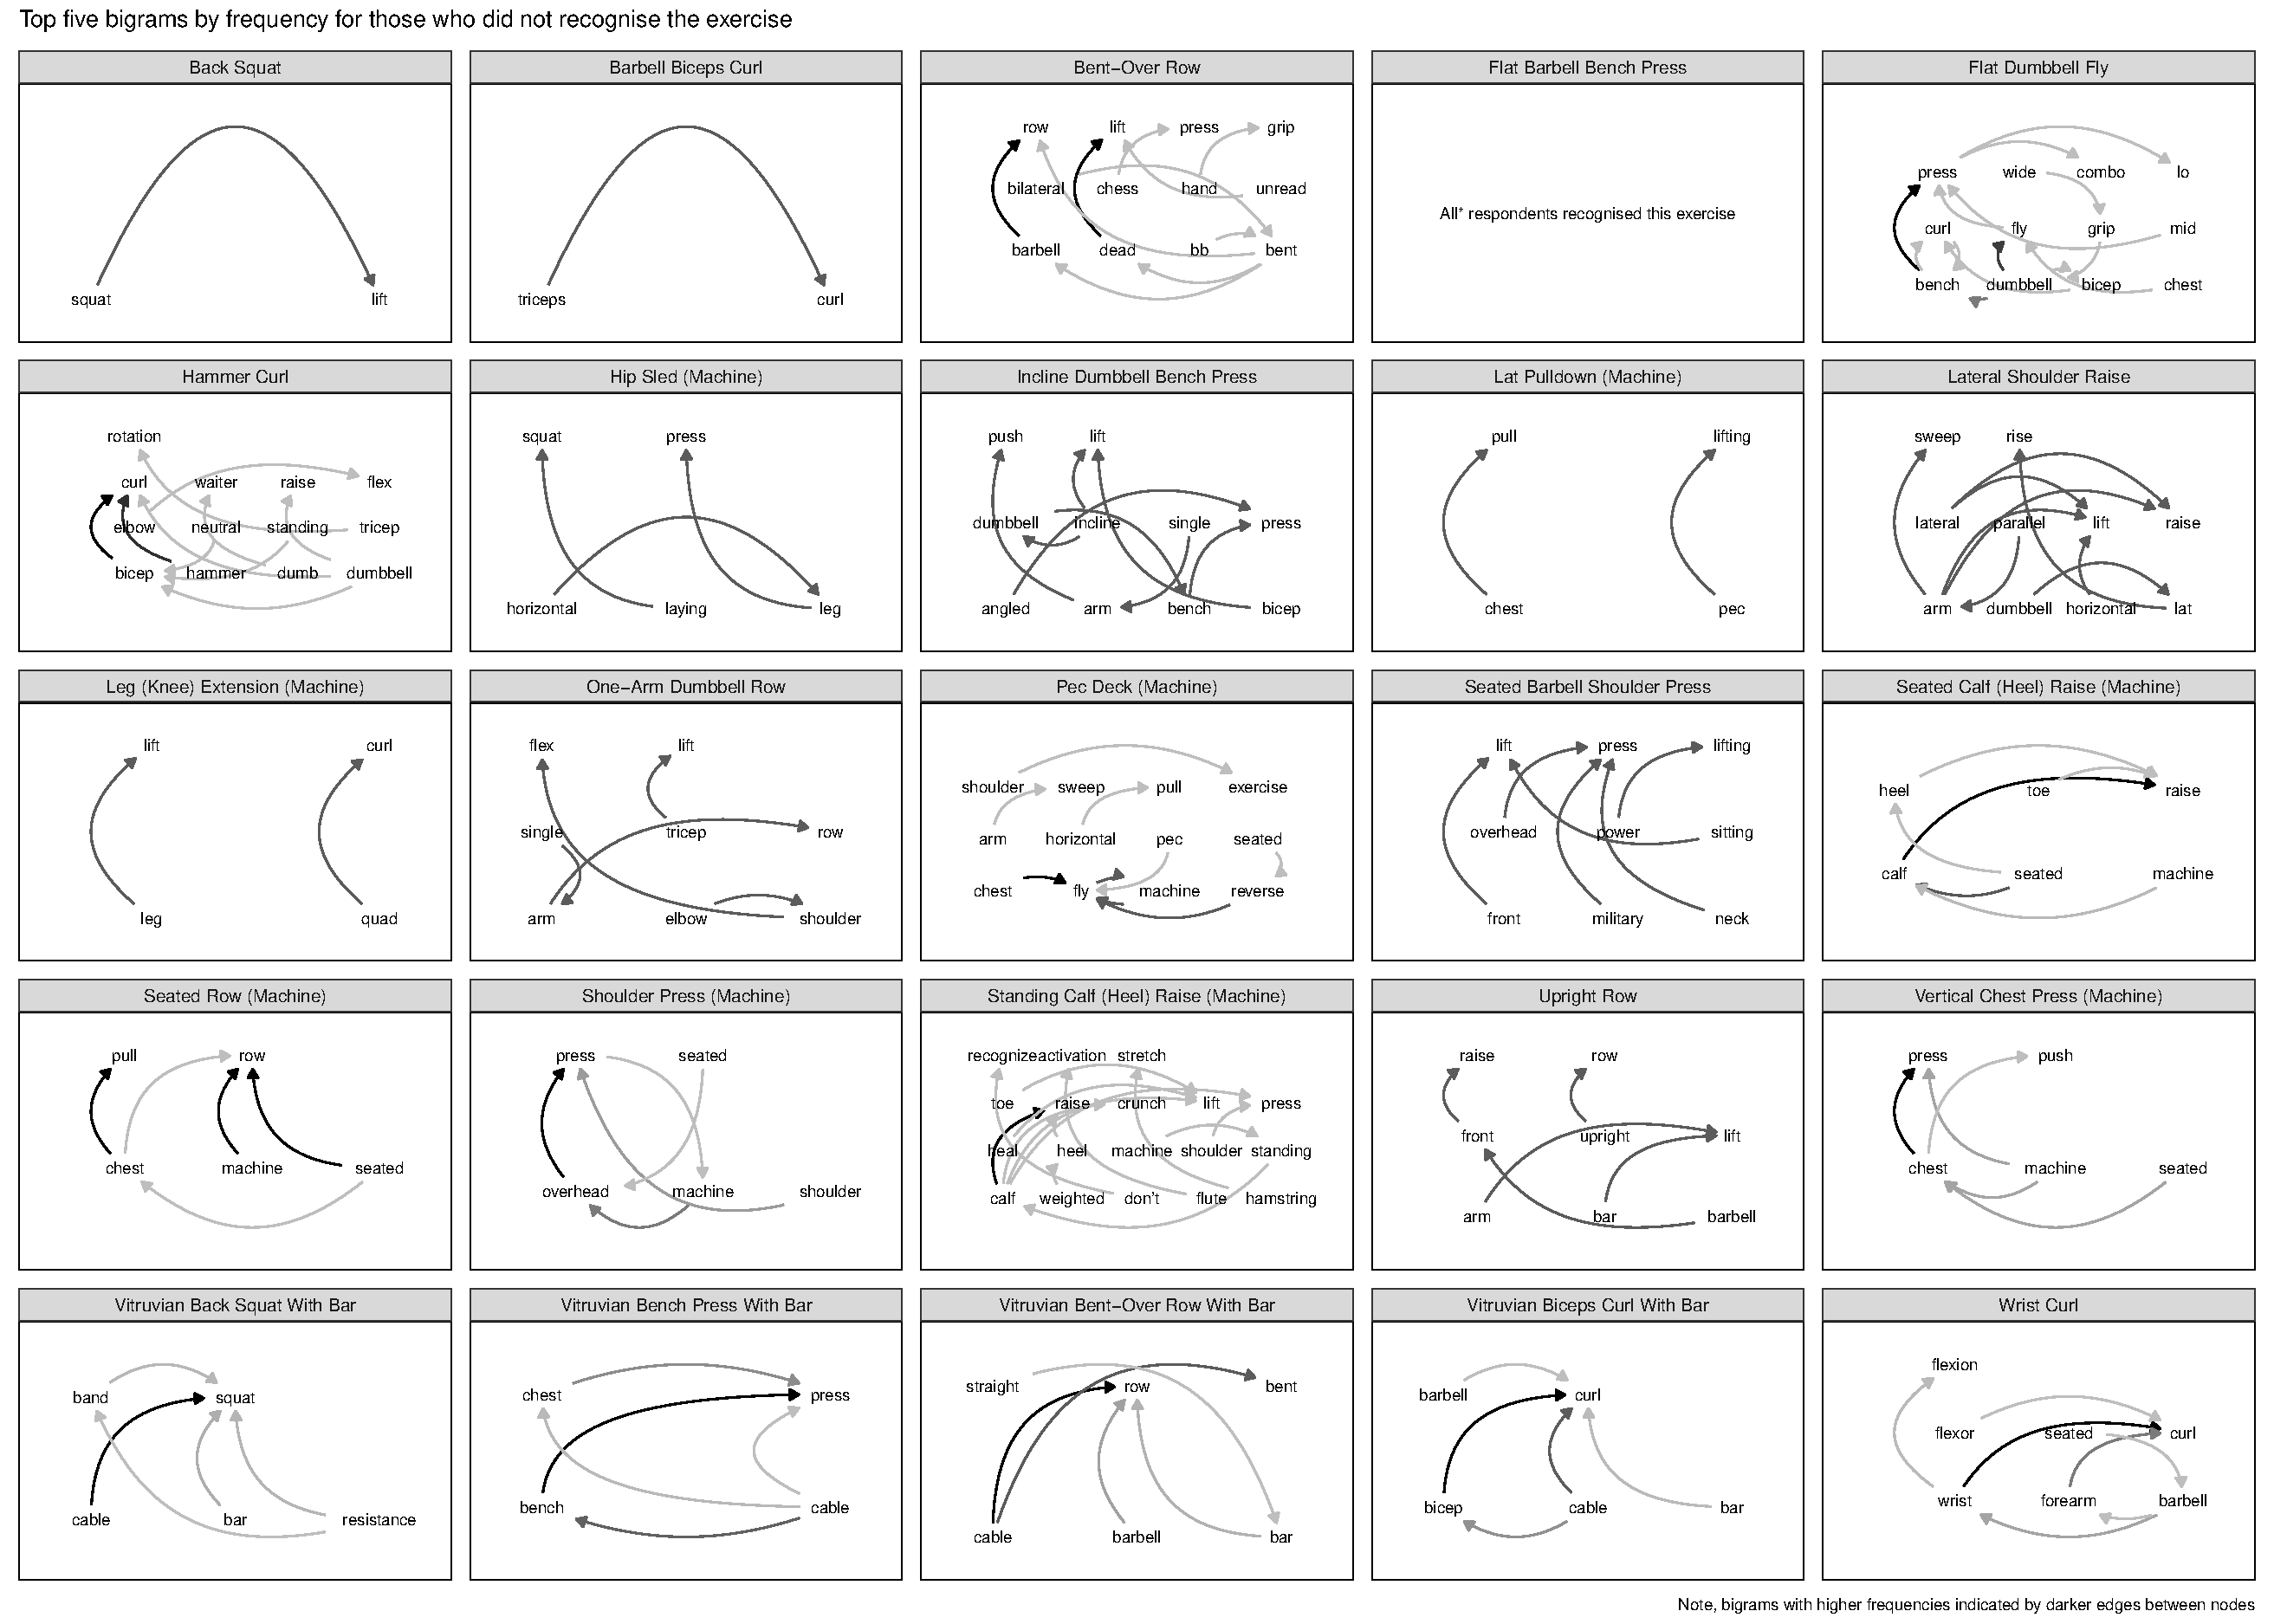
\includegraphics[keepaspectratio]{pre_print_files/figure-pdf/fig-bigram-not-recognise-plot-1.pdf}}

}

\caption{\label{fig-bigram-not-recognise-plot}Pairs of consecutive words
(bigrams) used in naming exercises by those who did not recognise the
exercise (note, names for exercises on each panel are the ``textbook''
names provided). *Only one respondent did not recognise the Flat Barbell
Bench Press exercise but responded with ``No'' as the name, hence there
being no bigrams for this.}

\end{figure}%

\end{landscape}

Lastly, the majority of participants agreed or strongly agreed that
exercise names are important (74\%), exercises are named inconsistently
(63\%), exercise names impact how information about exercise learned
(69\%), that they sometimes call the same exercise by different names
(73\%), and that a system standardizing exercise names would be
beneficial (69\%). The breakdown of responses can be seen in
Figure~\ref{fig-likert-plot}.

\begin{figure}

\centering{

\pandocbounded{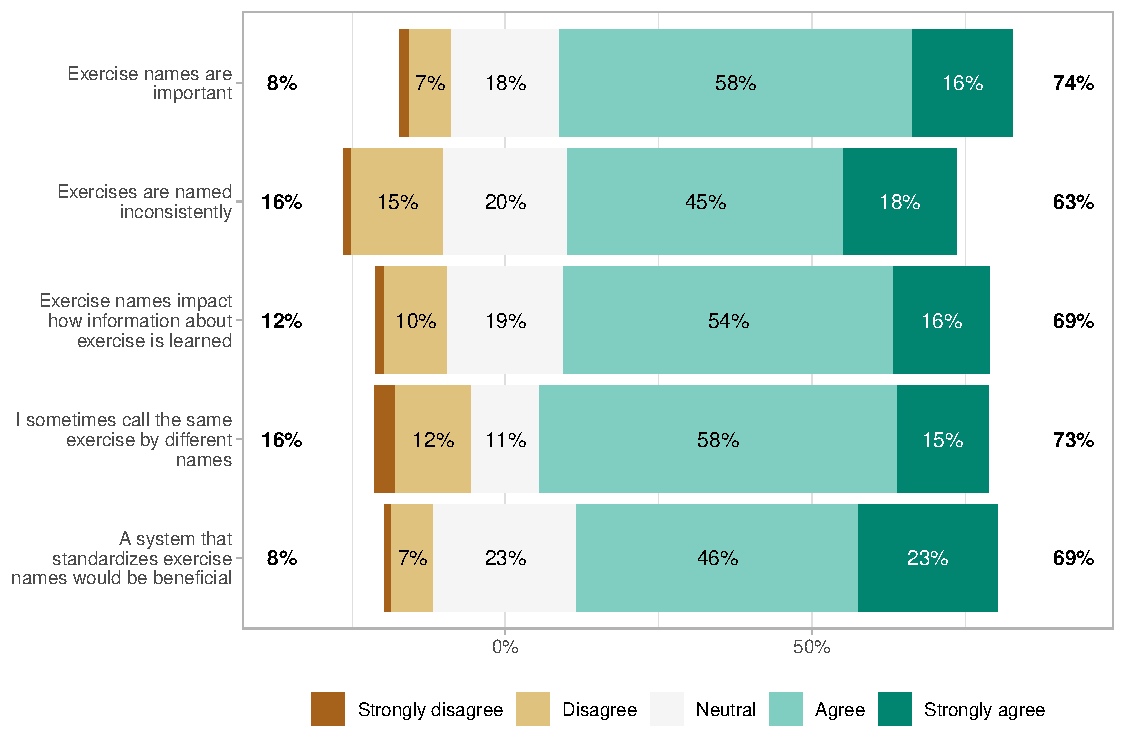
\includegraphics[keepaspectratio]{pre_print_files/figure-pdf/fig-likert-plot-1.pdf}}

}

\caption{\label{fig-likert-plot}Distribution of responses to each Likert
scale question.}

\end{figure}%

\section{Discussion}\label{discussion}

The findings of this study further support that naming conventions for
exercises are inconsistent (Jackson et al., 2013; Nuzzo, 2017, 2021).
However, whilst most exercises were widely recognised, recognition
influenced naming patterns: those who recognised exercises used more
consistent, commonly shared terminology, whereas unrecognised exercises
elicited more idiosyncratic naming. Equipment-related terms were
consistently important when applicable, but other naming components
(e.g., body position, body part, movement direction,
unilateral/bilateral execution) varied substantially in importance.
Bigrams showed that recognised exercises were typically labelled using
``textbook'' word pairings, while unrecognised exercises produced more
variable combinations. Participants generally agreed that exercise names
are important (74\%), inconsistently used (63\%), and influence learning
(69\%), many reported using multiple names for the same exercise (73\%),
and most supported standardization (69\%).

Term frequencies indicated quite clearly patterns resembling Zipf's
law-like distributions suggesting that exercise language follows broader
linguistic principles seen in natural language systems i.e., a small
number of highly common terms coexist with a long tail of infrequently
used variants. Indeed, our findings suggest that resistance exercise
naming may be an emergent, socially learned system rather than a
formally codified one and a result of cultural familiarity. Supporting
this was the distribution of term frequencies between those who did and
did not recognise exercises where the lack of long right tail for the
former suggested more commonly shared terms whereas the latter were more
likely to adopt idiosyncratic words. But, despite there being more
commonly used words by those who recognised exercises and also that
naming conventions appears to converge upon the ``textbook'' names used,
there was still considerable inconsistency within this group and the
majority of respondents also admitted that they use names
inconsistently. Indeed, given a significant proportion of respondents
were educated or working in the field of resistance training,
inconsistency may be a feature of language use in the field and not
merely due to unfamiliarity. This suggests that, within the folk
taxonomy of resistance exercise names, and groups that adopt this,
flexibility may not hamper communication and there is acceptance and
normalisation of naming flexibility.

Although there is evidently considerably variability in language,
emergent taxonomies and naming conventions still tend to adopt certain
principles of classification (Berlin, 1972; Berlin et al., 1973; Brown
et al., 1976). Within resistance exercise names there are a variety of
word types that have been shown to be adopted (Nuzzo, 2017). However,
although our results suggested that terms accurately identifying the
equipment were important when naming an exercise which used that
equipment, there was considerable variety in whether terms relating to
other word categories exercises were grouped by were important when
naming them (e.g., body position, body part, action performed, direction
of action, or whether bilateral/unilateral). This may indicate that
people prioritize equipment as the most visually or functionally salient
feature of an exercise when communicating about it. The inclusion of the
newly developed connected adaptive machines (i.e., Vitruvian) perhaps
support this as, the term frequency-inverse equipment frequency
suggested that the top five terms people used when attempting to name it
related to guesses as to what type of equipment it might be, based on
equipment terms that are already more familiar (e.g., \emph{``band''},
\emph{``cable''}; see \url{https://osf.io/c2zpj}).

Whilst these results suggest the existence of a folk taxonomy with
particular features already in use, the fact that there is considerable
inconsistency in naming conventions necessarily creates greater
opportunity for miscommunication and misunderstanding. It may be that
within public and applied settings and groups the terminology adopted by
individuals enables communication and understanding, but given the
applied nature of exercise science as a field there is
cross-communication that occurs between scientists and the public and
practitioners. Within textbooks and research articles exercises are
named inconsistently (Nuzzo, 2017, 2021) suggesting that scientists may
already share a similar taxonomy---a feature of which is indeed
inconsistency. However, different groups of exercise professionals may
use different taxonomies. Most respondents agreed that a system
standardising exercise names would be beneficial, but they also admitted
that they name exercises inconsistently. Singular terms are not a
necessary, but are a sufficient, condition for clear communication as it
is quite natural for synonyms to be used and understood by communities;
indeed our results suggest this may be the case as despite inconsistency
most do recognise and converge on similar naming conventions. The
results may support development of a hierarchical taxonomy rather than a
single \emph{``correct''} or \emph{``standard''} name for each exercise.
For example, exercises could be classified according to the word
categories previously highlighted (Nuzzo, 2017) with acceptable synonyms
nested within broader categories. This approach may be more realistic
than attempting to eliminate synonym use entirely, and it may facilitate
communication across different groups and settings.

Some limitations of the present study should be noted. Respondents to
our survey were predominantly English-speaking and experienced with
resistance exercise, either through education, employment, or their own
resistance exercise experience. As such, this limits the
generalisability of our findings to non-English speaking contexts and to
individuals who have limited exercise knowledge or experience. Exercises
were also presented to respondents as images and so the extent to which
recognition and understanding might occur in live, audio/conversational,
or purely written contexts is less clear. Future work could expand this
to such contexts and also explore longitudinal language development in
exercise nomenclature - e.g., through analyses of historical corpi.
Lastly, it is unclear whether any attempt at standardisation in the face
of the natural language use in these domains might improve communication
and understanding in public, applied, or scientific contexts. As such,
empirical work should be an essential part of any research programme
that intends to introduce exercise name standardisation. Indeed,
standardization may not be necessary for shared communication and
understanding.

\section{Conclusion}\label{conclusion}

Our findings suggest that naming of resistance exercise follows broad
linguistic principles (e.g., Zipf's law) and elements of a shared ``folk
taxonomy.''. Despite this, there was substantial inconsistency in
exercise naming practices. However, whilst such a folk taxonomy might
enable clear communication within public and applied settings, the
development of standardized terminology or a formal scientific taxonomy
might be warranted to ensure facilitation of communication and
understanding across domains and settings. Alternatively, a hierarchical
taxonomy and system of translation across synonyms in use already may be
a valuable pursuit. \# Funding Information

No direct funding was received for this study.

\section{Author Contributions}\label{author-contributions}

JN and JS conceived the idea for the project and designed the methods.
JN coordinated and oversaw the data collection including survey
distribution. JS conducted the statistical analyses and produced data
visualisations. JS drafted the initial manuscript. JN and JS contributed
to editing the manuscript and approved the final manuscript.

\section{Competing Interests}\label{competing-interests}

JN was previously employed at Vitruvian -- the company that designed the
connective adaptative resistance exercise machines that were featured in
some of the photographs in the current study.

JS provides research consultancy through his company Steele Research
Limited, is contracted currently by MacroFactor and Kieser Australia
through Steele Research Limited, and has also received travel expenses
and honoraria for speaking from fit20 International, Exercise School
Portugal, and Discover Strength.

The content does not necessarily represent the official views of the
affiliations or contracting organisations listed.

\section{Data and Supplementary Material
Accessibility}\label{data-and-supplementary-material-accessibility}

All data and code utilised for data preparation and analyses are
available in either the Open Science Framework page for this project
\url{https://osf.io/4uaqr/overview} or the corresponding GitHub
repository \url{https://github.com/jamessteeleii/exercise_names_survey}.

\section{References}\label{references}

\protect\phantomsection\label{refs}
\begin{CSLReferences}{1}{0}
\bibitem[\citeproctext]{ref-berlinSpeculationsGrowthEthnobotanical1972}
Berlin, B. (1972). Speculations on the {Growth} of {Ethnobotanical
Nomenclature}. \emph{Language in Society}, \emph{1}(1), 51--86.
\url{https://www.jstor.org/stable/4166669}

\bibitem[\citeproctext]{ref-berlinGeneralPrinciplesClassification1973}
Berlin, B., Breedlove, D. E., \& Raven, P. H. (1973). General
{Principles} of {Classification} and {Nomenclature} in {Folk Biology}.
\emph{American Anthropologist}, \emph{75}(1), 214--242.
\url{https://www.jstor.org/stable/672350}

\bibitem[\citeproctext]{ref-brownGeneralPrinciplesBiological1976}
Brown, C. H., Kolar, J., Torrey, B. J., Truong-Quang, T., \& Volkman, P.
(1976). Some general principles of biological and non-biological folk
classification. \emph{American Ethnologist}, \emph{3}(1), 73--85.
\url{https://doi.org/10.1525/ae.1976.3.1.02a00050}

\bibitem[\citeproctext]{ref-jacksonStandardizationNomenclatureResistance2013}
Jackson, M. C., Brown, L. E., Coburn, J. W., Judelson, D. A., \&
Cullen-Carroll, N. (2013). Towards standardization of the nomenclature
of resistance training exercises. \emph{Journal of Strength and
Conditioning Research}, \emph{27}(5), 1441--1449.
\url{https://doi.org/10.1519/JSC.0b013e318289168d}

\bibitem[\citeproctext]{ref-associationEssentialsStrengthTraining2016}
National Strength and Conditioning Association (NSCA). (2016).
\emph{Essentials of {Strength Training} and {Conditioning With Web
Resource} 4ed}. Human Kinetics.

\bibitem[\citeproctext]{ref-nuzzoWordsPatternsThat2017}
Nuzzo, J. L. (2017). Words and {Patterns That Comprise Resistance
Training Exercise Names}. \emph{Journal of Strength and Conditioning
Research}, \emph{31}(3), 826--830.
\url{https://doi.org/10.1519/JSC.0000000000000965}

\bibitem[\citeproctext]{ref-nuzzoInconsistentUseResistance2021}
Nuzzo, J. L. (2021). Inconsistent {Use} of {Resistance Exercise Names}
in {Research Articles}: {A Brief Note}. \emph{Journal of Strength and
Conditioning Research}, \emph{35}(12), 3518--3520.
\url{https://doi.org/10.1519/JSC.0000000000004083}

\bibitem[\citeproctext]{ref-nuzzoEccentricMuscleActions2023}
Nuzzo, J. L., \& Nosaka, K. (2023). Eccentric {Muscle Actions Add
Complexity} to an {Already Inconsistent Resistance Exercise
Nomenclature}. \emph{Sports Medicine - Open}, \emph{9}, 118.
\url{https://doi.org/10.1186/s40798-023-00667-4}

\bibitem[\citeproctext]{ref-nuzzoConnectiveAdaptiveResistance2023}
Nuzzo, J. L., Pinto, M. D., \& Nosaka, K. (2023). Connective {Adaptive
Resistance Exercise} ({CARE}) {Machines} for {Accentuated Eccentric} and
{Eccentric-Only Exercise}: {Introduction} to an {Emerging Concept}.
\emph{Sports Medicine}, \emph{53}(7), 1287--1300.
\url{https://doi.org/10.1007/s40279-023-01842-z}

\bibitem[\citeproctext]{ref-rodriguez-sanchezGratefulFacilitateCitation2023}
{Rodriguez-Sanchez, F., cre, cph, Jackson, C. P., Hutchins, S. D., \&
Clawson, J. M.} (2023). \emph{Grateful: {Facilitate Citation} of {R
Packages}}.

\bibitem[\citeproctext]{ref-winstonTwentyFirstCenturyBiological2018}
Winston, J. E. (2018). Twenty-{First Century Biological Nomenclature-The
Enduring Power} of {Names}. \emph{Integrative and Comparative Biology},
\emph{58}(6), 1122--1131. \url{https://doi.org/10.1093/icb/icy060}

\end{CSLReferences}




\end{document}
